A range query is a database operation that retrieves all the records that lies in a range. In this project, we perform range query on $2$-dimensional data only. In addition, we only consider a range query where the range is defined as a rectangle. Under these assumptions, a range query can be formalised as a query $\mathcal{Q}(\boldsymbol{l}, \boldsymbol{u})$ where $l,u\in\mathbb{R}^2$ and $split\_axis$ as $\mathcal{S}$.

\begin{mscexample}
	For example, assume we have the points
	$$
	[(1,2), (3,4), (3.5, 4), (5,6)]
	$$
	and the range query $\mathcal{Q}((2,3), (5,5))$, as shown below:
	
	\begin{minipage}[t]{\linewidth}
	\centering
   	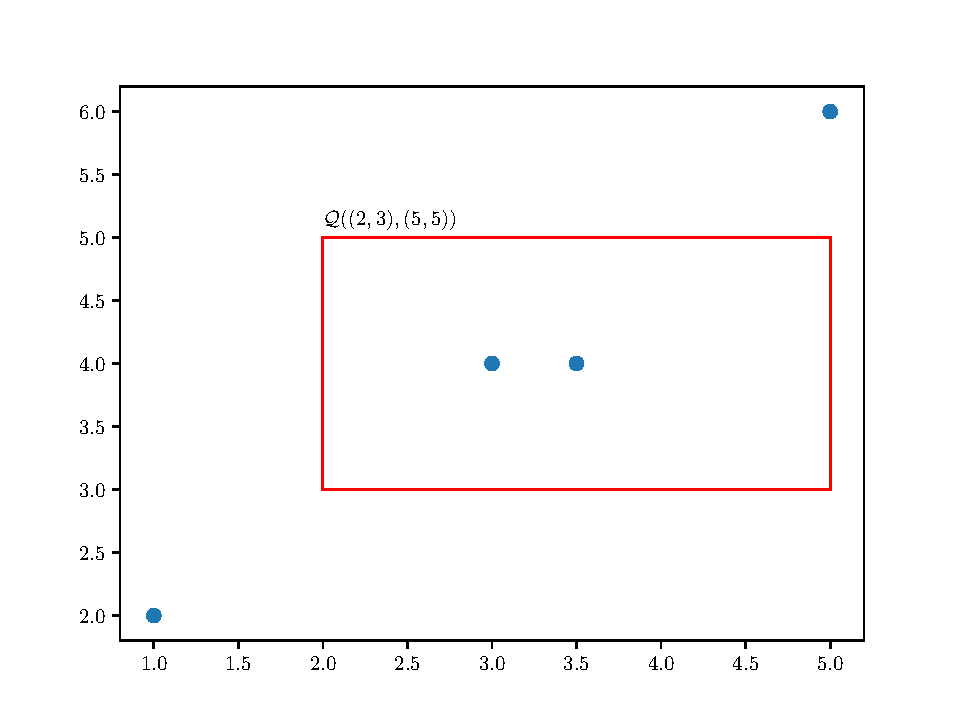
\includegraphics[width=10cm]{graphs/implementation/queries/range_query.pdf}
   	\label{fig:range_query_demo}
   	\captionof{figure}{A Range Query Example where $\mathcal{Q}(\boldsymbol{l}, \boldsymbol{u})=\mathcal{Q}((2,3),(5,5))$}
	\end{minipage}
	
In this example, the range query should return the points that lies inside the red rectangle, i.e. $((3,4), (3.5, 4))$.

\end{mscexample}

\subsubsection{Range Query with $K$D-Tree}

\begin{figure}[htp]
    \centering
    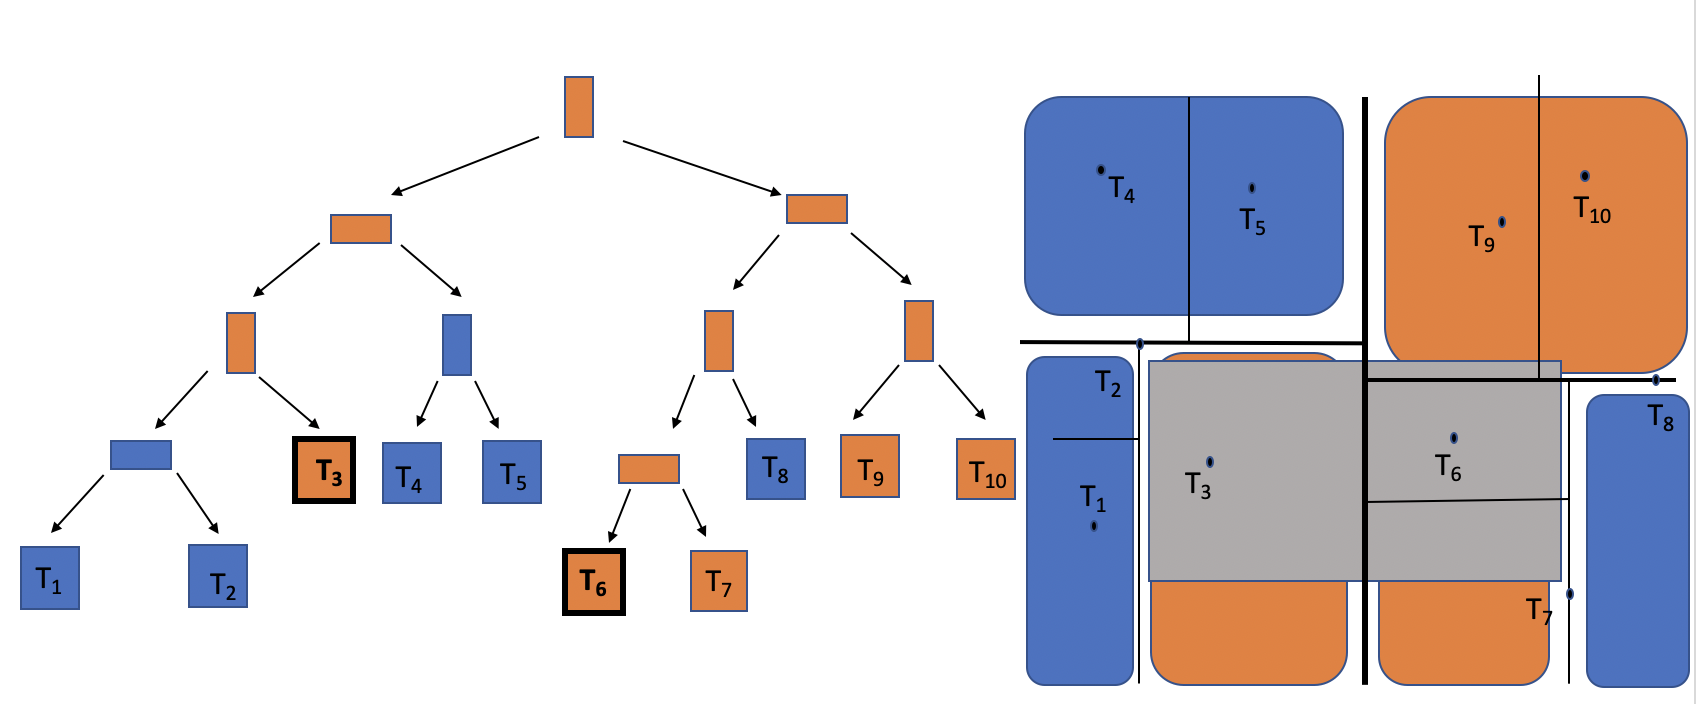
\includegraphics[width=1.0\textwidth]{graphs/KD_Tree_Range_Query_Algorithm.png}
    \caption{$K$D-Tree for Range Query Algorithm (Orange color are the visited points and blue color are the points not visited) 
    1) Tree representation of points. \\
    2) Subdivision of space into cells.(Orange color are the visited cells and blue color are the cells not visited) 
    }
    \label{fig:KD-Tree_for_Range_Query_Algorithm}
\end{figure}


% TODO: THIS ALGORITHM IS STILL NOT COMPLETE, and hard to follow.

% DONE: It is finished now.

\begin{algorithm}[H]
    \SetAlgoLined
    \SetKwInOut{Input}{Input}
    \SetKwInOut{Output}{Output}
    \Input{\texttt{Rectangle range (Lower;l and upper;u) $\mathcal{Q}(\boldsymbol{l}, \boldsymbol{u}); [l \in \mathbb{R};u \in \mathbb{R}]$}}
    \Output{\texttt{List of points within $\mathcal{Q}(\boldsymbol{l}, \boldsymbol{u})$}}
    % \texttt{SEARCH\_RANGE\_QUERY($\mathcal{Q}(\boldsymbol{l}, \boldsymbol{u})$)}\\
    \eIf{\texttt{node.leftChild is leaf}}
        {
            \If {$cell(v) \subseteq \mathcal{Q}(\boldsymbol{l}, \boldsymbol{u})$}
                {\texttt{add all points within cell to list}}
            \eIf {$cell(v) \cap \mathcal{Q}(\boldsymbol{l}, \boldsymbol{u}) = \varnothing$}
                {\texttt{add nothing to list}}
            {\texttt{add all points reported within $cell(v) \cap \mathcal{Q}(\boldsymbol{l}, \boldsymbol{u})$}}
        }
        {
            % \texttt{SEARCH\_RANGE\_QUERY($\mathcal{Q}(\boldsymbol{l}, \boldsymbol{u})$)} //Recursively function is called\\
            \texttt{Search subtree of $v$ recursively.}
        }
        
    \texttt{Similarly, steps are repeated for node.rightChild}
    
    \caption{Range Query Algorithm for $K$D-Tree}
    \label{Range_Query_Algorithm_$K$D-Tree}
\end{algorithm}

In algorithm \ref{Range_Query_Algorithm_$K$D-Tree} 

\begin{enumerate}
    \item On line $1$, start with the root of tree in the function SEARCH\_RANGE\_QUERY(). We pass $\mathcal{Q}(\boldsymbol{l})$ and $\mathcal{Q}(\boldsymbol{u})$ and check if the point at the root falls within $\mathcal{Q}(\boldsymbol{l}, \boldsymbol{u})$. If the point falls within $\mathcal{Q}(\boldsymbol{l}, \boldsymbol{u})$ then the point is added to the result list.
    
    \item Let $v$, $w$ be left and right children nodes.(Refer fig \ref{fig:KD-Tree_for_Range_Query_Algorithm} for space partition of space)
    
    \item On line $2$, after checking the root, $v$ of root is searched to see if it is a leaf node. Since $v$ is not a leaf node, a decision to traverse the right or left subtree is made by checking its x-axis, y-axis and $\mathcal{S}$. 
    
    \item On line $3$, check if the entire cell of $v$ lie within the range of $\mathcal{Q}(\boldsymbol{l}, \boldsymbol{u})$. If it does then add all the points to the result.
    
    \item On line $6$, check if there is no intersection of the cell of $v$ with the $\mathcal{Q}(\boldsymbol{l}, \boldsymbol{u})$. If there is no intersection then nothing is added to the result list.
    
    \item On line $8$, since there must be a partial intersection of the cell of $v$, add the points from the cell that lie within $\mathcal{Q}(\boldsymbol{l}, \boldsymbol{u})$. 
    
    \item On line $11$, keep traversing within the subtree as in above steps until we get all the points within $\mathcal{Q}(\boldsymbol{l}, \boldsymbol{u})$
    % \item In fig \ref{fig:KD-Tree_for_Range_Query_Algorithm} we can see that all cells that intersect $\mathcal{Q}(\boldsymbol{l}, \boldsymbol{u})$ are checked and all the cells that are not intersected by $\mathcal{Q}(\boldsymbol{l}, \boldsymbol{u})$ are pruned. This improves the performance of the range query and hence results in much faster query.\\
\end{enumerate}

There are two cases in range query search:
\begin{enumerate}
    \item\textbf{Case 1}: When an entire subtree lie within $\mathcal{Q}(\boldsymbol{l}, \boldsymbol{u})$.
    \item\textbf{Case 2}: When only a part of the subtree lie within $\mathcal{Q}(\boldsymbol{l}, \boldsymbol{u})$.
\end{enumerate}

\begin{mscexample}

    
    \begin{minipage}[t]{\linewidth}
    \centering
    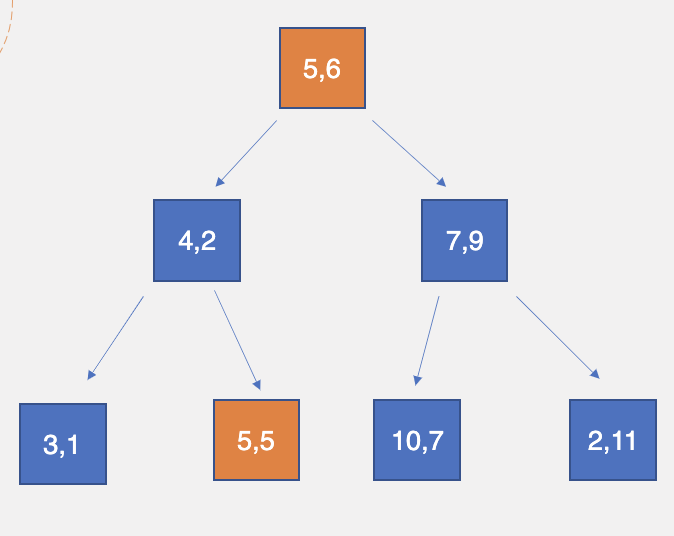
\includegraphics[width=6cm]{graphs/Range_Query_Tree.png}
    \label{fig:KD-Tree_for_Range Query}
    \hfill
    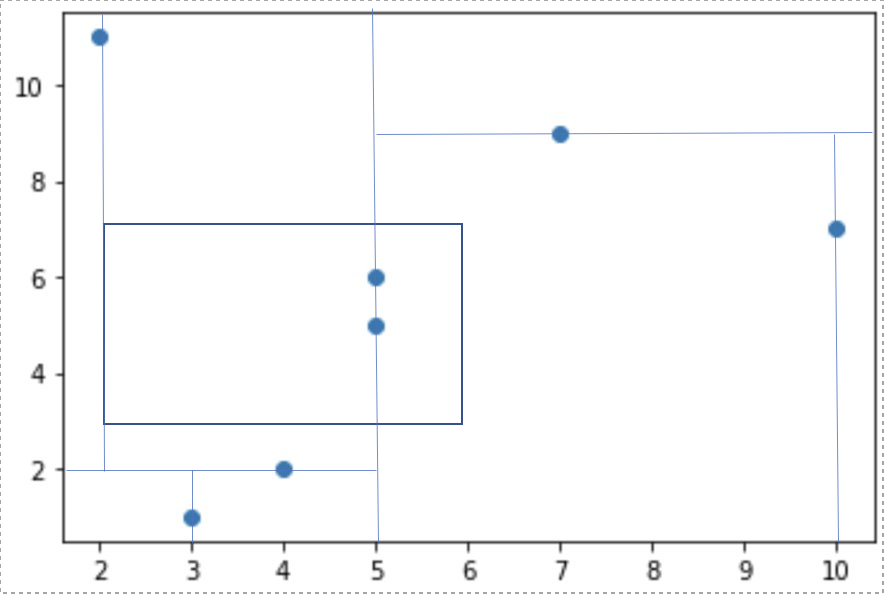
\includegraphics[width=6cm]{graphs/Range_Query_plot.png}
    \label{fig:KD_Tree_Range_Query_Plot}
    % \caption{Case 1: $K$D-Tree for Range Query (Case 1). Points highlighted in orange are returned in the query.}
    \end{minipage}


    
\begin{enumerate}
    \item\textbf{Case 1} : For example we have a tree with Point list as 
	$$[(5,6),(4,2),(7,9),(3,1),(5,5),(10,7),(2,11)]$$
	
	 with $\mathcal{Q}(\boldsymbol{l}) = (2,3)$ and $\mathcal{Q}(\boldsymbol{u}) = (6,7)$. \\
	 We follow below steps in order to get the results:
% 	 We can see the points along with $\mathcal{Q}(\boldsymbol{l}, \boldsymbol{u})$ plotted in \ref{fig:KD_Tree_Range_Query_Plot}.
	 \begin{enumerate}
	 
        \item Root point is checked and since its x-axis and y-axis both lie within $\mathcal{Q}(\boldsymbol{l}, \boldsymbol{u})$ i.e., $2 > 5 > 6$ and $3 > 6 > 7$, it is added to result list.
        
         \item In order to check whether to traverse left or right, we check if the x-axis($\mathcal{Q} = 0$) of root is greater than or equal to the $\mathcal{Q}(\boldsymbol{l}$) x-axis. Since this value is larger ($5 > 2$), it will then traverse to the left. 
         
         \item Increase $\mathcal{S}$ to $1$.
         
         \item We have root.leftChild to be $(4,2)$. Check if both the x-axis and y-axis lie within  $\mathcal{Q}(\boldsymbol{l}, \boldsymbol{u})$. Since the y-axis doesn't lie in $\mathcal{Q}(\boldsymbol{l}, \boldsymbol{u})$, this point is not added ($2 \notin [3,7]$). 
         
         \item Similarly, it keeps adding points to list while it recursively traverses the tree and checks if the points lie within $\mathcal{Q}(\boldsymbol{l}, \boldsymbol{u})$ until it reaches a leaf.
         
	\end{enumerate}
	\begin{minipage}[t]{\linewidth}
        \centering
        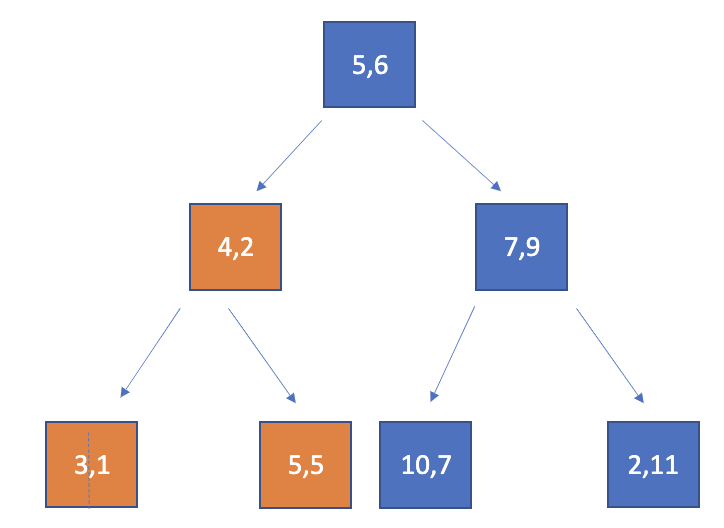
\includegraphics[width=6cm]{graphs/Range_Query_Tree_02.png}
        % \caption{Case 2: $K$D-Tree for Range Query. Points highlighted in orange are returned in the query.}
        \label{fig:KD-Tree_for_Range_Query_Case2}
        \hfill
        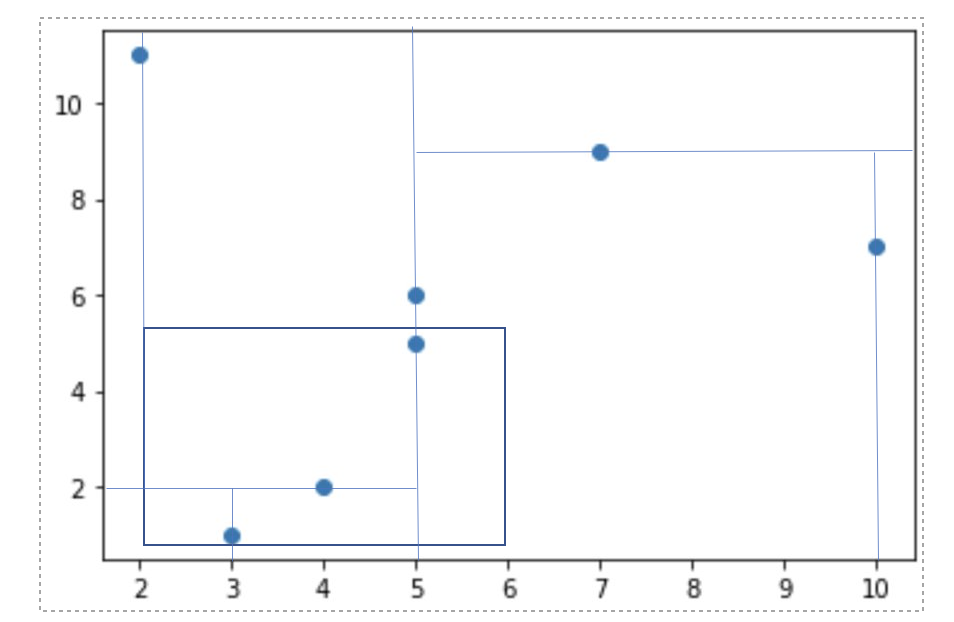
\includegraphics[width=6cm]{graphs/Range_Query_plot_02.png}
        % \caption{Case 2: $K$D-Tree Range Query Plot on 2-dimensional plane. Points $(4,2)$, $(3,1)$ and $(5,5)$ lie within $\mathcal{Q}(\boldsymbol{l}, \boldsymbol{u})$}
        \label{fig:KD_Tree_Range_Query_Plot_Case2}
        \end{minipage}
    
	 \item\textbf{Case 2} : For example, we have a tree with Point list as: 

	$$[(5,6),(4,2),(7,9),(3,1),(5,5),(10,7),(2,11)]$$
	
	with $\mathcal{Q}(\boldsymbol{l}) = (2,0.5)$ and $\mathcal{Q}(\boldsymbol{u}) = (6,4.75)$. \\
	We follow below steps in order to get the results:
% 	We can see the points along with $\mathcal{Q}(\boldsymbol{l}, \boldsymbol{u})$ plotted in \ref{fig:KD_Tree_Range_Query_Plot_Case2}.
	\begin{enumerate}
    	\item Root point is checked and since both x-axis and y-axis do not lie within $\mathcal{Q}(\boldsymbol{l}, \boldsymbol{u})$ i.e., $6 \notin [0.5, 4.75]$ it is not added to the list.
    	
    	\item In order to check whether to traverse left or right of the tree, we check if the x-axis of root is greater than or equal to $\mathcal{Q}(\boldsymbol{l})$ x-axis. Since the value is larger ($5 > 2$), it will then traverse to the left. Root.leftChild node is $(4,2)$. Since both, x-axis and y-axis lie within $\mathcal{Q}(\boldsymbol{l}, \boldsymbol{u})$, it is added to the result list. 
    	
    	\item Since all the points in this cell lie within $\mathcal{Q}(\boldsymbol{l}, \boldsymbol{u})$, they are all added to the list.
    	
    \end{enumerate}	
\end{enumerate}
\end{mscexample}

\begin{figure*}[t]
    \centering
    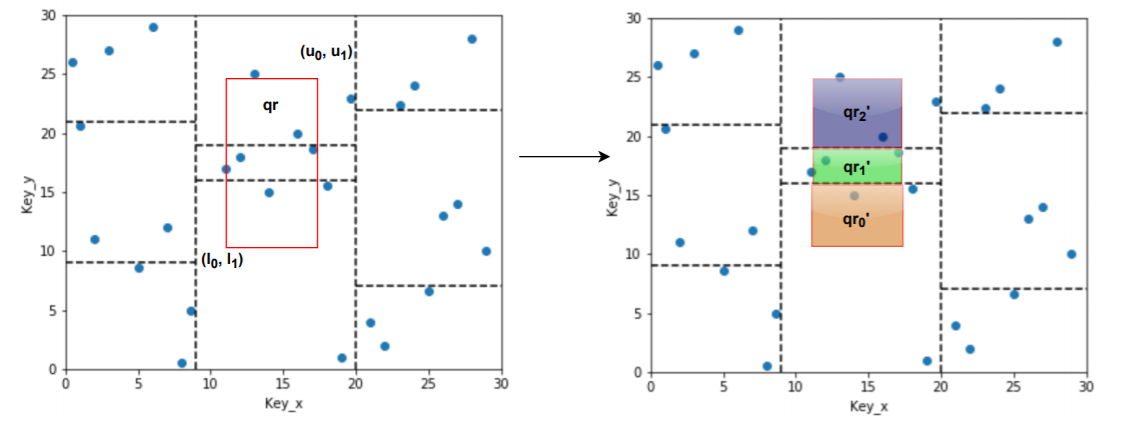
\includegraphics[width=1\textwidth]{graphs/range_query_lisa.png}
    \caption{Range Query Search in Lisa.
    1) Find the cells that overlap with $\mathcal{Q}(\boldsymbol{l}, \boldsymbol{u})$. \\
    2) Decompose $\mathcal{Q}(\boldsymbol{l}, \boldsymbol{u})$ into the unions of smaller query rectangles, each of which intersect only one cell. \\
    3) Find shards corresponding to lower and upper coordinates for each $\mathcal{Q}(\boldsymbol{l}, \boldsymbol{u})$, and perform a sequential search. }
    \label{fig:Range_Query_Lisa}
\end{figure*}


\subsubsection{Range Query with LISA}


For a range query $\mathcal{Q}(\boldsymbol{l},\boldsymbol{u})$, we first find the cells that overlap with $\mathcal{Q}$. Then we decompose $\mathcal{Q}$ into the union of smaller query rectangles $\bigcup \mathcal{Q}_i$ such that each smaller query rectangles intersects only one cell, as shown in the Fig. \ref{fig:Range_Query_Lisa}.



 Suppose that $\mathcal{Q}=\bigcup \mathcal{Q}_i$ where $\mathcal{Q}_i=[l_{i_0}, u_{i_o})\times [l_{i_1}, u_{i_1})$, i.e. we have $\mathcal{Q}_i$ representing the $i$th smaller query rectangles of one cell $C_j$.
 
 Then we can calculate the mapped values of $\mathcal{Q}_i$, i.e. $\mathcal{M}(l_{i_0}, l_{i_1})$ and $\mathcal{M}(u_{i_0}, u_{i_1})$. For simplicity, we use $m_l^{(i)}$ and $m_u^{(i)}$ to denote $\mathcal{M}(l_{i_0}, l_{i_1})$ and $\mathcal{M}(u_{i_0}, u_{i_1})$ respectively.
 
After creating corresponding mapped values, we then apply the shard prediction function $\mathcal{SP}(m_{l}^{i})$ and $\mathcal{SP}(m_{u}^{i})$ to predict the shard that could possibly contain keys that lie in the query rectangle $\mathcal{Q}_i$. Then in each shard, we perform a sequential search to find the desired keys. 

